\section{Simulation}

\subsection{Collapsed workflow}
\ididthis{Ettore Ricci, Paolo Palumbo, Francesco Boldrini}

\begin{figure}[H]
\centering
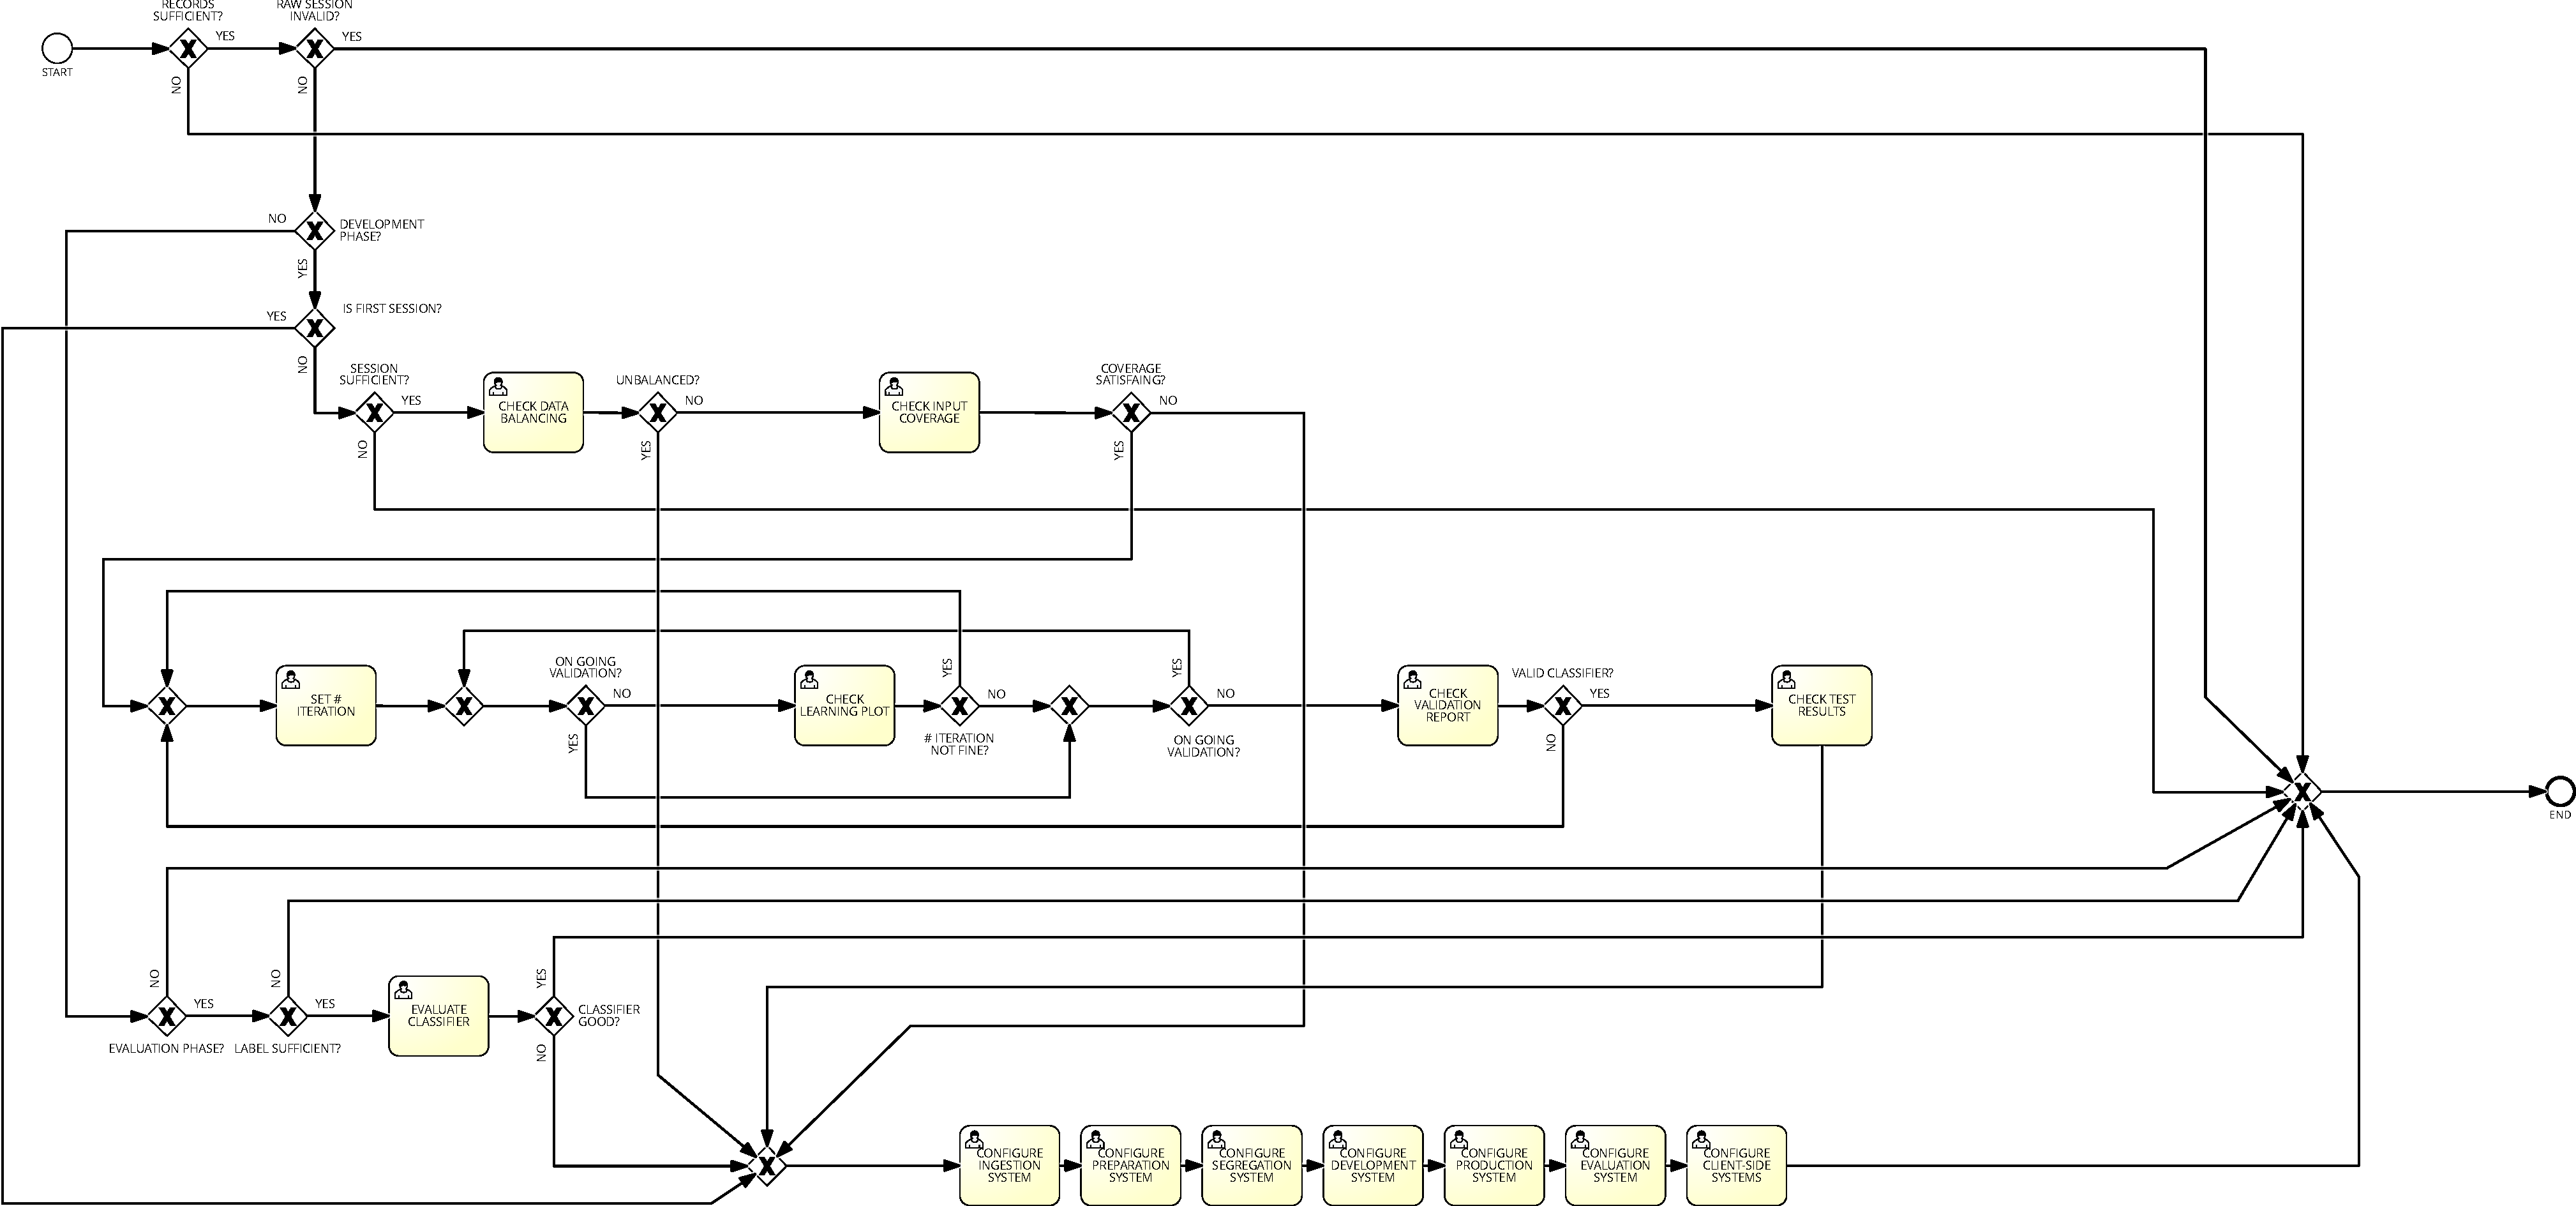
\includegraphics[width=0.8\textwidth]{figures/Collapsed Workflow SIM.pdf}
\caption{Collapsed workflow}
\label{fig:collapsed_workflow}
\end{figure}


NB: we set the total number of process instances to 6852,\\
as with our assumptions for the two initial gates, where\\
we discard 10\% of the sessions twice, we need 6852 sessions\\
to start, to work with the dictaded assumptions of the 5550\\
good sessions of the documentation.\\


\begin{table}[H]
    \centering
    \begin{tabularx}{\textwidth}{|X|c|c|c|}
    \hline
    \textbf{Parameter} & \textbf{\% of the Gate} & \textbf{Motivation} \\
    \hline
     \# Iteration not fine? & 20\% & According to the assumptions of the \\
     & & documentation, we set the \% of iters \\
     & & that are not fine to 20\% \\
    \hline
    Classifier Good? & 86\% & According to the assumptions of the \\
     & & docs, classifiers are good 86 of the time \\
    \hline
    Coverage satisfying? & 33\% & According to the assumptions of the \\
     & & docs, coverage is satisfying 33\% of the time \\
    \hline
    Development Phase? & 9\% & In this gate, out of 5550, 500 are \\
     & & in the development phase \\
    \hline
    Is First Session? & 1\% & In this gate, out of 500, 1 is 
    \\ & & in the first session, but the gate
    \\ & & won't load less than 1\% on BIMP 
    \\
    \hline
    Labels sufficient? & 71\% & Given 5550 good sessions, and 
    \\ & & assuming that those will yields
    \\ & & 5 proper classifiers, given the 
    \\ & & probabilities at the preceeding 
    \\ & & gates and the rounding because of 
    \\ & & necessity of the gate to have at 
    \\ & & least 1\% as value, we 
    \\ & & need to have 71\% of the sessions 
    \\ & & to have sufficient labels to respect 
    \\ & & the documentation's assumptions.
    \\
    \hline
    On going Validation? & 90\% & We set validation to 90\% as most
    \\ & & of the times this step involves the
    \\ & & autonomous systems and not humans \\
    \hline
    Raw session Invald? & 10\% & We assume that 90\% of the times
    \\ & & the raw session is valid.\\
    \hline
    Records Sufficient? & 90\% & We assume that 90\% of the times
    \\ & & the records are sufficient.\\
    \hline
    Session Sufficient? & 99\% & We set sessions sufficient to 99\% as
    \\ & & with the document's assumptions, we 
    \\ & & would need roughly 545 sessions to 
    \\ & & have 5 final good classifiers and here
    \\ & &  we already start with 500, which is
    \\ & & already lower than what we would need.\\
    \hline
    Unbalanced? & 20\% & The documentation assumes that
    \\ & &  20\% of the classes are balanced\\
    \hline
    Valid Classifier? & 95\% & The documentation assumes that
    \\ & &  95\% of the classifiers are valid\\
    \hline

\end{tabularx}
\end{table}
